\section{Results}
For testing the three implementations we used a 30 second bathymetry grid as the baseline input dataset. 
Execution times were recorded by using each programming paradigm’s underlying method for getting current time at application start and application end, subtracting these values and converting to hours. 
From prior work done in the past we had access to a single threaded Fortran program that computes mean and standard deviation for gridded data.  
We used the Fortran execution times previously previously recorded for 30 second input data to compare against our results.  
While not an ideal comparison, time constraints prevented us from creating single threaded versions of our implementations and running them.  
They simply take too long to process a data set as large as the 30 second resolution grid that we used as our baseline.

\par
The Mean and Standard deviation times are shown in Figure 3.
All results were timed in hours for each coresponding core ammount.
As to be expected, the mean and standard deviation graphs fit the classical parallel efficency curve \cite{buzbee}.
Figure 3 does not include results for the MPI implementation because of the impediments discussed earlier in the report.
\begin{figure}[h]
    \centering
    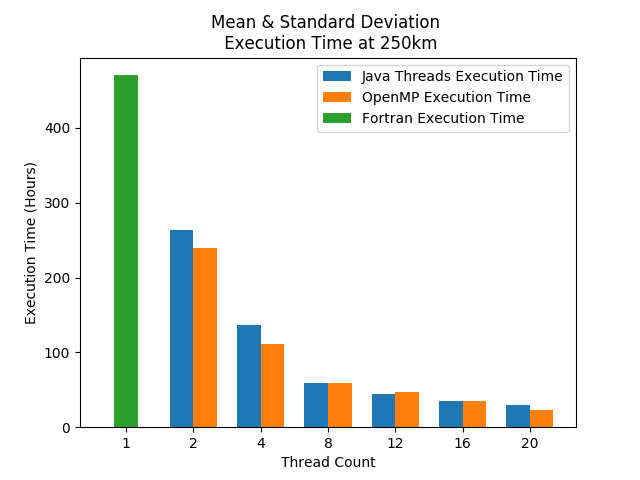
\includegraphics[scale=0.5]{merp}
    \caption{Results for Mean and Standard Deviation}
    \label{fig:3}
\end{figure}

\par
Java threads preformed marginally slower than the C implementation.
However, this slow down scaled as more cores are used in computation.
Going from several days to only several hours at higher core counts.


\par
The Plane fit execution times are shown in Figure 4.
The original Fortran program required months to run.
However, we timed the Java implementation at around two weeks for 20 cores.
We did not run it at lower core counts for lack of time.
Predicting based on a classic parallel computing trend line, the time requirements will be several months to compute those results.

\begin{figure}[h]
    \centering
    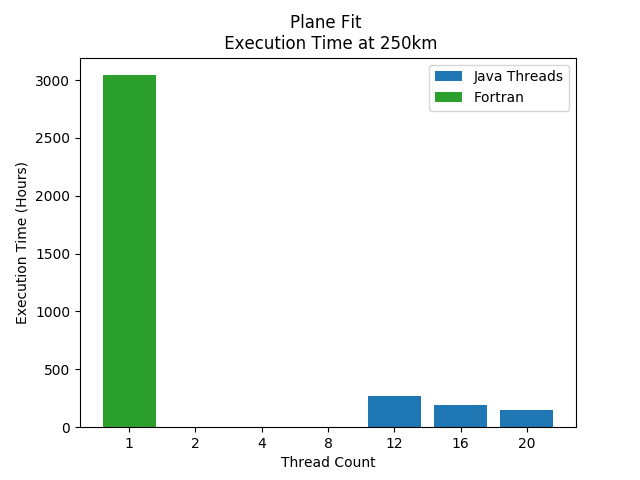
\includegraphics[scale=0.5]{plane}
    \caption{Results for Plane Fit}
    \label{fig:4}
\end{figure}

